\chapter{Conclusiones y Trabajos futuros}

%%%%%%%%%%%%%%%%%%%%%%%%%%%%%%%%%%%%%%%%%%%%%%%%
\section{Conclusiones}

En este trabajo, presentamos un sistema CAOS de planificaci\'on preoperatoria para fracturas en los miembros inferiores. Al mismo tiempo se cre\'o una nueva variante del algoritmo de deformaci\'on de im\'agenes basado en la t\'ecnica de MLS el cual es explicado detalladamente en el Cap\'itulo \ref{ourapproach}. Nuestro trabajo fue utilizado y probado por los miembros del Servicio de Traumatolog\'ia y Ortopedia del Hospital Universitario de Caracas (HUC) \cite{REF_HUC} para la planificaci\'on de m\'as de 100 casos de fracturas de miembros inferiores. Para emplear la propuesta aqu\'i planteada solo se requiere de al menos un computador (sin ning\'un requerimiento especial de hardware) y una c\'amara.

Para el momento del planteamiento del problema no se contaba con dispositivos de adquisici\'on de Rayos-X de forma digital. En este trabajo se plante\'o c\'omo emplear una c\'amara como dispositivo de adquisici\'on de im\'agenes en formato digital. En nuestras pruebas se emplearon diversas c\'amaras con resoluciones de al menos $3.15$ megap\'ixeles, con una dimensi\'on m\'axima de captura de $2048 \times 1536$ p\'ixeles. En este trabajo se presentaron y describieron todas las variables a tomar en cuenta para la adquisici\'on de la placa de Rayos-X en formato digital: ubicaci\'on del negatoscopio con respecto a la c\'amara, distancia de la c\'amara a la placa y el \'angulo formado con respecto a la placa. Todas las im\'agenes fueron capturadas satisfactoriamente.

Una vez capturada la placa de Rayos-X con la c\'amara, es necesario aplicar un proceso de calibraci\'on para obtener la correspondencia entre p\'ixeles y mil\'imetros. Este trabajo plante\'o una soluci\'on empleando una herramienta simple: una perforadora de orificio. Se present\'o el Algoritmo de B\'usqueda de Orificios (descrito en el subsecci\'on \ref{AlgBusqOri1}) donde se explica detalladamente cada par\'ametro necesario para la calibraci\'on de las im\'agenes capturadas. El algoritmo de calibraci\'on de im\'agenes radiogr\'aficas fue presentado como un reporte t\'ecnico en una publicaci\'on interna de la Escuela de Computaci\'on - UCV \cite{RAM_TEC10}.

En este trabajo tambi\'en se present\'o una nueva variante para la deformaci\'on de im\'agenes empleando la t\'ecnica de MLS. Con nuestra t\'ecnica se obtiene una deformaci\'on similar al doblado del implante realizado por el m\'edico cirujano dentro de un quir\'ofano. Se demostr\'o que al restringir el movimiento de los controladores de la deformaci\'on empleando un OBB se evitan posibles errores causados por el cirujano. Al mismo tiempo, los controladores son colocados de forma autom\'atica a lo largo del implante. El movimiento libre de los controladores puede causar distorsiones notables que cambiar\'ian las proporciones del implante. Esto es un factor no deseado para nuestra propuesta y es por ello la restricci\'on aplicada.

Por otro lado, se determin\'o de forma autom\'atica la resoluci\'on del mallado para la deformaci\'on de cada implante. En las pruebas realizadas, encontramos que un valor adecuado para la resoluci\'on del mallado es un $5\%$ de la longitud del eje mayor del implante. Con este valor es posible conseguir buenos resultados visuales y mantener la deformaci\'on en tiempo real sin afectar considerablemente el rendimiento de la aplicaci\'on.

En este trabajo se propone una nueva funci\'on de peso para la t\'ecnica MLS de deformaci\'on de im\'agenes. Cuando se compara con la funci\'on original propuesta en el trabajo de Schaefer et al. \cite{SCHAF06}, la nueva funci\'on ofrece resultados m\'as realistas para nuestro sistema de planificaci\'on preoperatoria para fracturas en los miembros inferiores. Se demostr\'o que para obtener dichos resultados, se requiere un valor de $k$ igual o superior a $2.5$. Este nuevo enfoque de nuestro trabajo fue desarrollado como una investigaci\'on novedosa y ser\'a presentada en una Conferencia Internacional, ver \cite{RAM11}. 

Seg\'un los estudios realizados se determin\'o que el tiempo de planificaci\'on empleando nuestra propuesta es menor que al realizar la planificaci\'on convencional en aproximadamente 28 minutos. Como se mostr\'o en la Tabla \ref{tab:timesp}, al realizar la planificaci\'on de manera convencional se requiere de una inversi\'on de de aproximadamente $45.9$ min. por parte del cirujano. Particularmente, la etapa de segmentaci\'on y ensamblaje de la fractura requiere de una mayor inversi\'on de tiempo, ver Tabla \ref{tab:porc}. El tiempo de esta etapa es proporcional a la complejidad de la fractura.

Con nuestra propuesta el tiempo de construcci\'on de una planificaci\'on se reduce en un $61\%$ en promedio con respecto a la planificaci\'on convencional. Parte de esta ganancia de tiempo se debe a la facilidad al utilizar las herramientas ofrecidas por nuestro sistema CAOS como las anotaciones, medidas con regla, \'angulos y c\'irculos, selecci\'on de un implante desde una librer\'ia y uso de la biblioteca de AO, as\'i como su almacenamiento para un posterior estudio. De lo anterior se puede concluir claramente que la planificaci\'on preoperatoria digital permite ahorrar tiempo en el quir\'ofano para los cirujanos. Esto es debido a que solamente se llevar\'a a un paciente a la sala de operaci\'on si se cuenta con todo el material necesario que se conocer\'a a priori.

El sistema CAOS presentado en este trabajo tambi\'en puede ser empleado como una aplicaci\'on did\'actica para los m\'edicos en formaci\'on. Los m\'edicos en formaci\'on o los m\'edicos realizando estudios especializados en el \'area de Traumatolog\'ia tendr\'an una gu\'ia para el estudio de casos cl\'inicos y para la construcci\'on de planificaciones preoperatorias a ser revisadas por especialistas.

La soluci\'on propuesta es un primer avance en Venezuela en el desarrollo de aplicaciones para planificaci\'on prequir\'urgica para fracturas. Actualmente, se encuentra en mejoramiento continuo, producto de la retroalimentaci\'on obtenida por parte del grupo de m\'edicos traumat\'ologos que lo est\'an empleando. Dicha informaci\'on permite entonces tomar en cuenta factores importantes para el mejoramiento en un futuro.

%%%%%%%%%%%%%%%%%%%%%%%%%%%%%%%%%%%%%%%%%%%%%%%%
\section{Trabajos futuros}

Se propone como trabajo futuro la creaci\'on de nuevos implantes para que el sistema CAOS no solo pueda aplicarse en planificaciones preoperatorias de miembros inferiores, sino para otros huesos tambi\'en. 

Adem\'as, el esquema presentado no es limitativo en cuanto a las etapas presentadas. En ciertas planificaciones preoperatorias (por ejemplo de pr\'otesis de cadera) es indispensable tener un m\'odulo de medici\'on de esfuerzo del peso del paciente sobre la pr\'otesis. Esta operaci\'on debe realizarse una vez colocado y fijado el implante, despu\'es de la etapa de deformaci\'on del implante. En este caso, se le podr\'ia agregar al sistema f\'acilmente una nueva etapa de c\'alculo de esfuerzo. 

Actualmente, el procesamiento y deformaci\'on en tiempo real de los implantes utilizados no genera mucha latencia. Si se utilizan implantes de mayor tama\~no (e.g. una pr\'otesis de cadera) el tiempo de respuesta puede ser mayor. Para evitar esto se propone crear un esquema adaptativo de subdivisi\'on del mallado, con una malla no uniforme con mayor resoluci\'on en los sectores donde se necesita una deformaci\'on m\'as precisa y menor resoluci\'on donde se requiera menos precisi\'on. Esto se ilustra en la Figura \ref{fig:distMul}.
\begin{figure}[htbp]
  \begin{center} 
  \subfigure[]{\label{fig:distan1}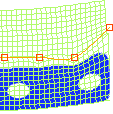
\includegraphics[width=0.30\columnwidth]{images/distance3.png}} \hspace{1.0cm}  \subfigure[]{\label{fig:distan2}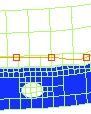
\includegraphics[width=0.25\columnwidth]{images/distancemulti.png}}
  \end{center}
  \caption{(a) Mallado uniforme empleado en nuestra propuesta (b) Mallado adaptativo propuesto como trabajo futuro}
  \label{fig:distMul}
\end{figure}

Otro trabajo futuro, es la posibilidad de leer im\'agenes de Rayos-X en formato DICOM \cite{REF_DICOM}. En este caso, no es necesario realizar los orificios con la perforadora de papel porque la calibraci\'on se obtiene al momento de la adquisici\'on y la informaci\'on de esto se encuentra dentro de la cabecera del archivo.

Por \'ultimo, una mejora para facilitar y acelerar la deformaci\'on de los implantes por parte de los cirujanos es permitir que los controladores tengan influencia sobre sus controladores vecinos, para que cuando se mueva un controlador influya en una cierta proporci\'on a sus controladores vecinos. De esta forma los controladores vecinos se mover\'an autom\'aticamente hacia la misma direcci\'on que el controlador seleccionado.